\chapter{Kalibrierung}

Die Lochkamera ist eine M\"oglichkeit, um Bilder von Gegenst\"anden zu erzeugen. Ein primitiver Aufbau besteht aus einem geschlossenen Geh\"ause mit einer runden \"Offnung auf einer Seite. Auf der gegen\"uberliegenden Seite befindet sich ein ebener Bildsensor um das einfallende Licht als Bild aufzunehmen. In Abbildung \ref{fig:calibration_pinhole} ist die Funktionsweise einer Lochkamera schematisch dargestellt. Die Kamera dient dazu einen dreidimensionalen Punkt auf einer zweidimensionalen Ebene durch Projektion abzubilden.



\begin{figure}
 \centering
 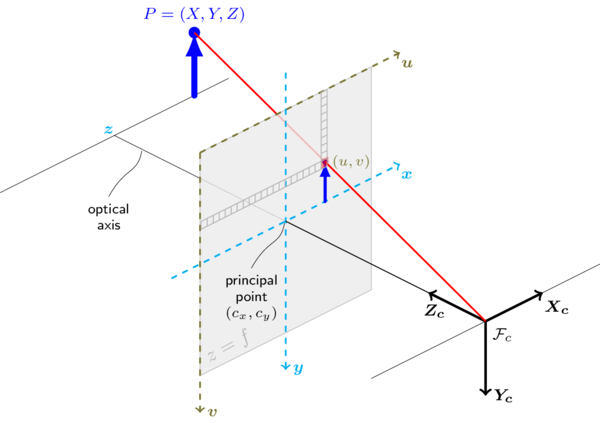
\includegraphics[width=1\textwidth]{media/calibration/pinhole_camera_model.png}
 \caption{Kalibrierung - Modell der Lochkamera}
 \label{fig:calibration_pinhole}
\end{figure}

Die Projektion l\"asst sich dabei darstellen als:
\begin{equation}
 w
 \begin{pmatrix}
  u \\ v \\ 1
 \end{pmatrix}
 = A \begin{pmatrix}
    X \\ Y \\ Z \\ 1
   \end{pmatrix}
   =
 = K \begin{bmatrix}
      R | t
     \end{bmatrix}
   \begin{pmatrix}
    X \\ Y \\ Z \\ 1
   \end{pmatrix}
\end{equation}

Der Punkt \( P \in \mathbb{R}^3, P = (X, Y, Z) \) wird hierbei auf den Punkt \( P' \in \mathbb{R}^2, P' = (u, v) \) projeziert. Die Projektionsmatrix \( A \) muss folglich die Dimension \(4 \times 3 \) aufweisen und wird aus der intrinsischen Kameramatrix \(K \in {R}^{3 \times 3} \) und der zusammengesetzten extrinsischen Kameramatrix \( \begin{bmatrix}
      R | t
  \end{bmatrix} \in \mathbb{R}^{3 \times 4} \) gebildet.

\begin{multicols}{2}
\centering

\begin{equation}
 K = \begin{pmatrix}
      f_x & 0 & c_x \\
      0 & f_y & c_y \\
      0 & 0 & 1
     \end{pmatrix}
\end{equation}

\columnbreak
\centering
\begin{equation}
  \begin{bmatrix}
      R | t
  \end{bmatrix}
  = 
  \begin{pmatrix}
   r_{11} & r_{12} & r_{13} & t_1 \\
   r_{21} & r_{22} & r_{23} & t_2 \\
   r_{31} & r_{32} & r_{33} & t_3 
  \end{pmatrix}
\end{equation}
\end{multicols}

Die intrinsische Matrix enth\"alt die Brennweiten \( (f_x, f_y) \) der Kamera sowie die Koordinaten des Bildmittelpunkts \( (c_x, c_y) \).
Die extrensische Matrix enth\"alt die Rotationsmatrix \( R \in \mathbb{R}^{3 \times 3} \) sowie den Translationsvektor \( t \in \mathbb{R}^3 \).

Da es durch Verzerrungen noch zu unerw\"unschten Effekten bei der Bildaufnahme kommen kann wird das Modell um einige Verzerrungskoeffizienten erweitert. Die Auswirkungen der radialen und tangentialen Verzerrung k\"onnen in den Abbildungen \ref{fig:calibration_radial} und \ref{fig:calibration_tangential} betrachtet werden. 

\begin{figure}
 \centering
 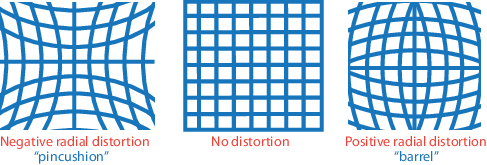
\includegraphics[width=1\textwidth]{media/calibration/calibration_radial_distortion.png}
 \caption{Kalibrierung - Radiale Verzerrung}
 \label{fig:calibration_radial}
\end{figure}

\begin{figure}
 \centering
 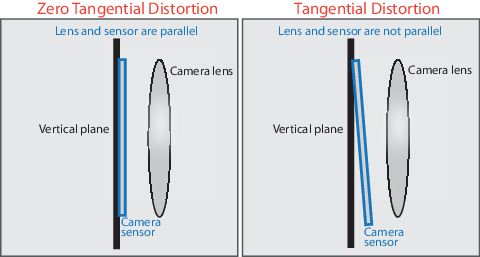
\includegraphics[width=1\textwidth]{media/calibration/calibration_tangentialdistortion.png}
 \caption{Kalibrierung - Tangentiale Verzerrung}
 \label{fig:calibration_tangential}
\end{figure}


\begin{multicols}{2}
\centering
Radiale Verzerrung \\
Koeffizienten: \( k \in \mathbb{R}^3 = \begin{pmatrix} k_1 & k_2 & k_3 \end{pmatrix}^\intercal \) \\
\(r^2=x^2+y^2 \) \\
\begin{eqnarray*}
x_{radial} &=& x(1+k_1r^2+k_2r^4+k_3r^6) \\
y_{radial} &=& y(1+k_1r^2+k_2r^4+k_3r^6)
\end{eqnarray*}

\columnbreak
\centering
Tangentiale Verzerrung \\
Koeffizienten: \( p \in \mathbb{R}^2 = \begin{pmatrix} p_1 & p_2 \end{pmatrix} ^\intercal \) \\
\(r^2=x^2+y^2 \) \\
\begin{eqnarray*}
 x_{tangential} &=& x+[2p_1xy+p_2(r^2+2x^2)] \\
 y_{tangential} &=& y+[p_1(r^2+2y^2)+2p_2xy]
\end{eqnarray*}
\end{multicols}


\section{Kamera Kalibrierung}

Bei im Handel erh\"altlichen Kameras sind die Kameraparameter h\"aufig nicht angegeben oder auch zu ungenau f\"ur wissenschaftliche Zwecke. Aus diesem Grund m\"ussen die Parameter durch einen Kalibriervorgang bestimmt werden. Ein Verfahren hierzu ist das Aufstellen eines linearen Gleichungssystems, welches durch die Abbildung bekannter dreidimensionaler Punkte in die Ebene erzeugt wird:
Es seien Kalibrierungsdaten \(X_i \in \mathbb{R}^3 \mapsto x_i \in \mathbb{R}^2, i \in \{1..m\} \) vorhanden. Gesucht ist die Kameramatrix \( P\in \mathbb{R}^{4 \times 3} \) sodass gilt: \( PX_i=x_i,  \forall i \in \{1..m\} \). Im Allgemeinen enth\"alt \(P\) 12 unabh\"angige Parameter, weshalb f\"ur das L\"osen des Gleichungssystems mindestens 12 Kalibrierungspunkte vorhanden sein m\"ussen. Bei dieser Anzahl ist das Gleichungssystem quadratisch und kann exakt gel\"ost werden. Bei einer h\"oheren Anzahl an Kalibrierungsdaten ist das Gleichungssystem \"uberbestimmt und besitzt somit keine eindeutige L\"osung mehr. Eine L\"osung des \"uberbestimmten Gleichungssystems kann beispielsweise durch die Gau\ss{}sche Normalenform oder die QR-Zerlegung gel\"ost werden. Die so berechnete L\"osung ist im Allgemeinen stabiler als die exakte L\"osung, da Fehler in den Eingangsdaten ausgeglichen werden.

\section{Stereokalibrierung}

F\"ur die Kalibrierung einer einzelnen Kamera sind die extrnisischen Kameradaten zumeist relativ uninteressant. Bei Stereosystem aus zwei Kameras ist jedoch die Ausrichtung beider Kameras zueinander von au\ss{}erordenlticher Relevanz, da hierdurch die Grundlage zur Disparit\"atsberechnung geschaffen wird. 

\begin{figure}
 \centering
 
\includegraphics[width=1\textwidth]{media/calibration/stereo_calibration2.png}
 \caption{Kalibrierung - Stereo Kalibrierung}
 \label{fig:calibration_radial}
\end{figure}

\section{Rektifizierung}

Bearbeiten der Bilder so, dass Epipolarlinien auf beiden Bildern parallel und in gleicher Zeile
